\documentclass{article}
\usepackage{graphicx}
\graphicspath{ {images/} }

% Math-mode symbol & verbatim
\def\W#1#2{$#1{#2}$ &\tt\string#1\string{#2\string}}
\def\X#1{$#1$ &\tt\string#1}
\def\Y#1{$\big#1$ &\tt\string#1}
\def\Z#1{\tt\string#1}
 
\newcommand\tab[1][1cm]{\hspace*{#1}}

\begin{document}

\title{%
  Advanced Nature Inspired Search and Optimisation  \\
  \large CA 2: Airline crew scheduling using GA  \\
    }

\author{1429527}

\maketitle

\section{The Algorithm}

This genetic algorythm will be used to solve the 'Airline Crew Schduling' problem where the cost needs to be minimused while traveling each leg of the journey.
\smallbreak
To implement the algorithm, I used the code given \cite{Shan} as the basis for my algorithm and added the required functionality on top. 
\smallbreak
The basis of the algorithm is to randomly initilise the population of a specified size, then use the top parents to produce offspring. Stochastic Ranking was used to find the fittest parents, then crossover, mutation and heuristic improvement was applied to produce the offspring. Heuristic improvement changed any columns which can be changed - i.e. more than one row is covered by the currently selected row, then filling in any gaps in the solution with minimal cost. Finally the top population size number of individuals from the original population and the offspring are selected to be the new population. 
\smallbreak
The Stochastic Ranking not only ranks by fitness, but penalises any violation by a set amount. It also introduces randomness in that swaps can occour if a value is higher than a threshold, without the penalty being smaller.
\smallbreak
Below is a graph plotting the current, best solution against the iteration number for benchmark sppnw41.

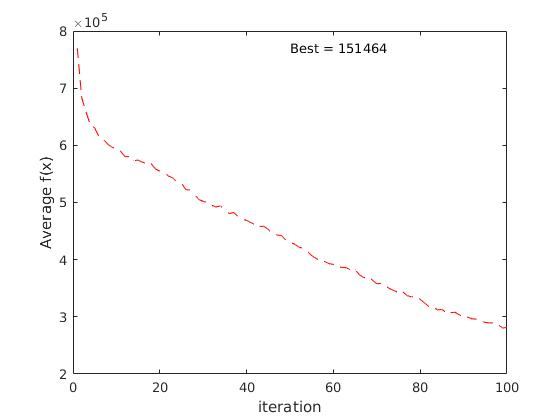
\includegraphics[width=10cm,height=10cm,keepaspectratio]{41Graph}

Below is the flow chart for the algorithm, containing sudo code given in \cite{1&3} and \cite{2}.
\smallbreak

\includegraphics[width=15cm,height=25cm,keepaspectratio]{Ex2-1}

\section{Benchmark Problem}

Number of runs: 10
\smallbreak
Population size: 200
\smallbreak
Max Iteration: 1000
\smallbreak
Violation penalty = 0.45

\subsection{sppnw41.txt}

\begin{center}
\begin{tabular}{ |c|c|c| } 
 \hline
Run & Min Cost & Constraint Violations \\ 
 \hline
 1 & 13218 & 0 \\ 
 \hline
 2 & 14253 & 0 \\ 
 \hline
 3 & 12663 & 0 \\ 
 \hline
 4 & 13209 & 0 \\ 
 \hline
 5 & 13572 & 0 \\ 
 \hline
 6 & 12663 & 0 \\ 
 \hline
 7 & 11679 & 0 \\  
 \hline
 8 & 12897 & 0 \\ 
 \hline
 9 & 13663 & 0 \\ 
 \hline
 10 & 14253 & 0 \\ 
 \hline
\end{tabular}
\end{center}

Average Result: 13204
\smallbreak
Average Violation: 0
\smallbreak
Standard Deviation: 785.4421

\subsection{sppnw42.txt}

\begin{center}
\begin{tabular}{ |c|c|c| } 
 \hline
Run & Min Cost & Constraint Violations \\ 
 \hline
 1 & 11598 & 1 \\ 
 \hline
 2 & 12210 & 0 \\ 
 \hline
 3 & 16656 & 1 \\ 
 \hline
 4 & 11544 & 0 \\ 
 \hline
 5 & 12114 & 2\\ 
 \hline
 6 & 11260 & 1 \\ 
 \hline
 7 & 11828 & 1 \\  
 \hline
 8 & 11430 & 0 \\ 
 \hline
 9 & 6940 & 2 \\ 
 \hline
 10 & 11272 & 0 \\ 
 \hline
\end{tabular}
\end{center}

Average Result: 11685
\smallbreak
Average Violation: 0.8
\smallbreak
Standard Deviation: 2313

\subsection{sppnw43.txt}

\begin{center}
\begin{tabular}{ |c|c|c| } 
 \hline
Run & Min Cost & Constraint Violations \\ 
 \hline
 1 & 8890 & 1 \\ 
 \hline
 2 & 12018 & 0 \\ 
 \hline
 3 & 11330 & 0 \\ 
 \hline
 4 & 14076 & 0 \\ 
 \hline
 5 & 10650 & 0 \\ 
 \hline
 6 & 11036 & 0 \\ 
 \hline
 7 & 10912 & 0 \\  
 \hline
 8 & 12090 & 0 \\ 
 \hline
 9 & 14576 & 0 \\ 
 \hline
 10 & 14666 & 0 \\ 
 \hline
\end{tabular}
\end{center}

Average Result: 12024
\smallbreak
Average Violation: 0.1
\smallbreak
Standard Deviation: 1889

\section{Ranking Comparisons}

\cite{1&3} uses a Ranking Replacement strategy to order and ultimatly discard unfit individuals whereas the above, along with \cite{2} uses Stochastic Ranking. 
\smallbreak
Ranking replacement considers both the fitness (quality) and unfitness (feasibility) of the soluitons. It divides the current population into four groups compared to the offspring: G1 less fit and more unfit, G2 more fit and less unfit, G3 less fit anf more unfit and G4 more fit and less unfit. The offspring then replaces the member of a group with the worst unfitness, in that order - if G1 is empty, it will replace an item in G2 and so on. 
\smallbreak
Stochastic Ranking only compares the fitness of individuals. Probablity is introduced to allow infeasible options to be compared with those feasible; If both are feasible then the probability of comparing their fitness is 1 else it is $P_f$. This method comes from the need to balance the objective function are penalty function as so will most likely be more useful that Replacement Ranking if the penalty function is high. All items in the population and the offspring are compared in this way and then the bottom ranking (least fit) individuals are discarded so that the population remains at a constant size.
\smallbreak
With both menthods, care needs to be taken so that duplicte solutions are not entered as this limits the algorithm's ability to generate new solutions. However with Replacemnt Ranking, it appears that the offspring must always be entered into the new population even if it is worse than all items in the current population whereas Stochastic will reject all worse solutions regardless of when they were created.  
\smallbreak
Stochastic ranking will most likely be more computationally efficient as it will ahve the same complexity as bubble-sort on which it is based. Replacement Ranking requires the entire population to be split into four sections wuth respect to the offspring trying to be replaced, meaning popSize computations for every offspring; This amy be efficienct if the number of offspring is small.
\smallbreak
Replacement ranking dictates the item to be replaced by an offspring, however Stochastic ranking, as it has the variable Pt, can change the weight of infeasible solutions over time. This means that, as time goes on, the chance of an infeasible solution being carried forward can be reduced so as to focus on the current local optima. Ranking is designed to keep the scope of the solutoins broard and does not have such a variable to create an adaptive algorithm. 
 

\begin{thebibliography}{1}

\bibitem{1&3}
P.C. Chu, J.E. Beasley, Constraint Handling in Genetic Algorithms: The Set Partitioning Problem, Journal of Heuristics, 11: 323–357 (1998). 

\bibitem{2}
T.P. Runarsson, X. Yao Stochastic ranking for constrained evolutionary optimization, IEEE Trans. on Evolutionary Computation, 4(3): 284-294 (2000).

\bibitem{Shan}
S. He. Week 6 Lab Code Examples. (2016)

\end{thebibliography}
\end{document}


